% Created by tikzDevice version 0.12.6 on 2025-11-05 12:08:49
% !TEX encoding = UTF-8 Unicode
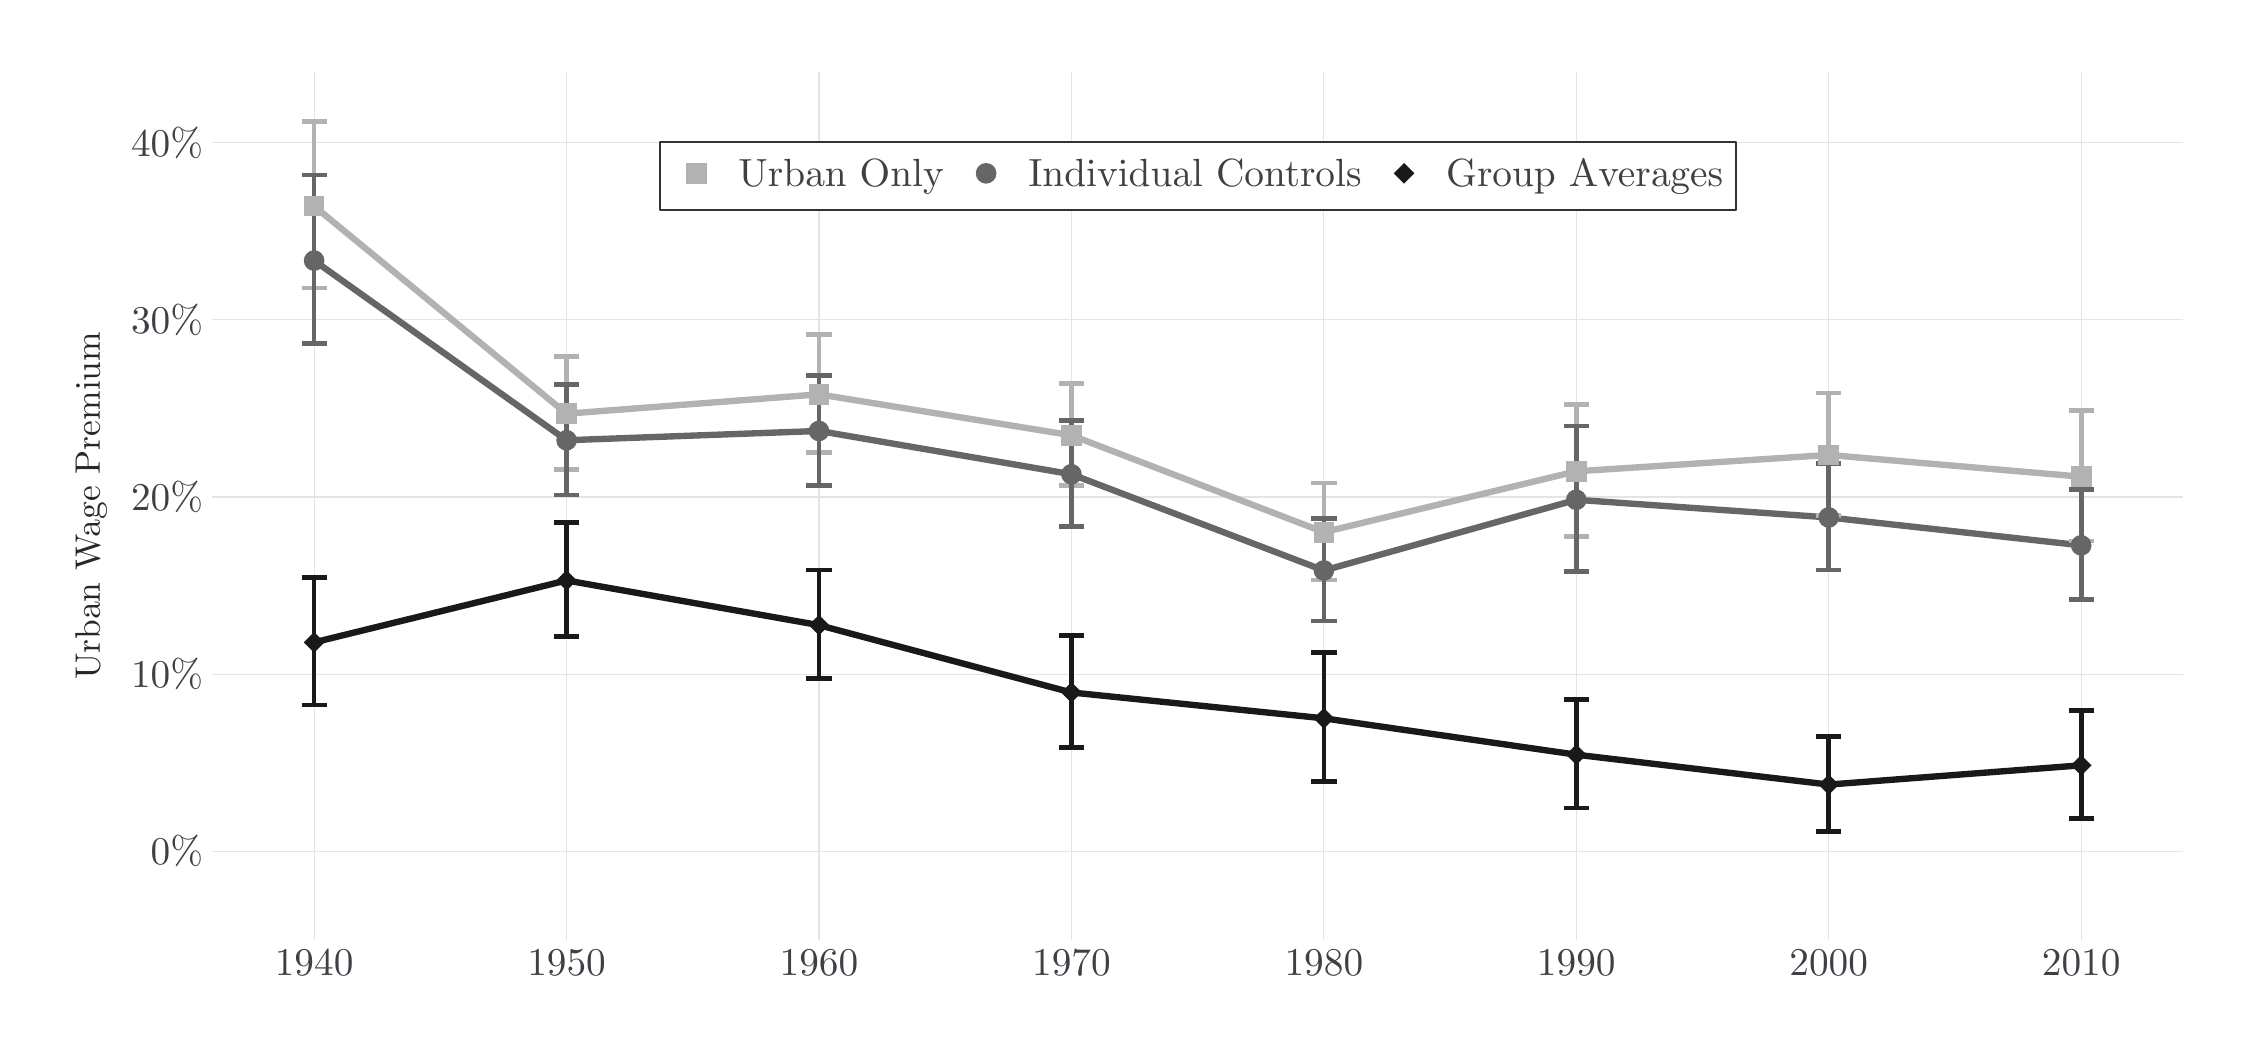
\begin{tikzpicture}[x=1pt,y=1pt]
\definecolor{fillColor}{RGB}{255,255,255}
\path[use as bounding box,fill=fillColor] (0,0) rectangle (794.97,361.35);
\begin{scope}
\path[clip] (  0.00,  0.00) rectangle (794.97,361.35);
\definecolor{drawColor}{RGB}{255,255,255}

\path[draw=drawColor,line width= 0.8pt,line join=round,line cap=round,fill=fillColor] (  0.00,  0.00) rectangle (794.97,361.35);
\end{scope}
\begin{scope}
\path[clip] ( 66.57, 31.76) rectangle (778.97,345.35);
\definecolor{drawColor}{RGB}{255,255,255}
\definecolor{fillColor}{RGB}{255,255,255}

\path[draw=drawColor,line width= 0.8pt,line join=round,line cap=round,fill=fillColor] ( 66.57, 31.76) rectangle (778.97,345.35);
\definecolor{drawColor}{RGB}{228,228,231}

\path[draw=drawColor,line width= 0.4pt,line join=round] ( 66.57, 63.76) --
	(778.97, 63.76);

\path[draw=drawColor,line width= 0.4pt,line join=round] ( 66.57,127.76) --
	(778.97,127.76);

\path[draw=drawColor,line width= 0.4pt,line join=round] ( 66.57,191.75) --
	(778.97,191.75);

\path[draw=drawColor,line width= 0.4pt,line join=round] ( 66.57,255.75) --
	(778.97,255.75);

\path[draw=drawColor,line width= 0.4pt,line join=round] ( 66.57,319.75) --
	(778.97,319.75);

\path[draw=drawColor,line width= 0.4pt,line join=round] (103.51, 31.76) --
	(103.51,345.35);

\path[draw=drawColor,line width= 0.4pt,line join=round] (194.73, 31.76) --
	(194.73,345.35);

\path[draw=drawColor,line width= 0.4pt,line join=round] (285.94, 31.76) --
	(285.94,345.35);

\path[draw=drawColor,line width= 0.4pt,line join=round] (377.16, 31.76) --
	(377.16,345.35);

\path[draw=drawColor,line width= 0.4pt,line join=round] (468.38, 31.76) --
	(468.38,345.35);

\path[draw=drawColor,line width= 0.4pt,line join=round] (559.59, 31.76) --
	(559.59,345.35);

\path[draw=drawColor,line width= 0.4pt,line join=round] (650.81, 31.76) --
	(650.81,345.35);

\path[draw=drawColor,line width= 0.4pt,line join=round] (742.03, 31.76) --
	(742.03,345.35);
\definecolor{drawColor}{gray}{0.70}

\path[draw=drawColor,line width= 2.3pt,line join=round] (103.51,296.85) --
	(194.73,221.85) --
	(285.94,228.85) --
	(377.16,214.05) --
	(468.38,179.04) --
	(559.59,201.04) --
	(650.81,206.95) --
	(742.03,199.10);
\definecolor{drawColor}{gray}{0.40}

\path[draw=drawColor,line width= 2.3pt,line join=round] (103.51,277.18) --
	(194.73,212.26) --
	(285.94,215.62) --
	(377.16,199.98) --
	(468.38,165.21) --
	(559.59,190.75) --
	(650.81,184.37) --
	(742.03,174.29);
\definecolor{drawColor}{gray}{0.10}

\path[draw=drawColor,line width= 2.3pt,line join=round] (103.51,139.23) --
	(194.73,161.61) --
	(285.94,145.45) --
	(377.16,121.12) --
	(468.38,111.78) --
	(559.59, 98.64) --
	(650.81, 87.84) --
	(742.03, 94.80);
\definecolor{drawColor}{gray}{0.70}

\path[draw=drawColor,line width= 1.7pt,line join=round] ( 98.95,327.45) --
	(108.07,327.45);

\path[draw=drawColor,line width= 1.7pt,line join=round] (103.51,327.45) --
	(103.51,267.28);

\path[draw=drawColor,line width= 1.7pt,line join=round] ( 98.95,267.28) --
	(108.07,267.28);
\definecolor{drawColor}{gray}{0.40}

\path[draw=drawColor,line width= 1.7pt,line join=round] ( 98.95,308.10) --
	(108.07,308.10);

\path[draw=drawColor,line width= 1.7pt,line join=round] (103.51,308.10) --
	(103.51,247.34);

\path[draw=drawColor,line width= 1.7pt,line join=round] ( 98.95,247.34) --
	(108.07,247.34);
\definecolor{drawColor}{gray}{0.10}

\path[draw=drawColor,line width= 1.7pt,line join=round] ( 98.95,162.60) --
	(108.07,162.60);

\path[draw=drawColor,line width= 1.7pt,line join=round] (103.51,162.60) --
	(103.51,116.59);

\path[draw=drawColor,line width= 1.7pt,line join=round] ( 98.95,116.59) --
	(108.07,116.59);
\definecolor{drawColor}{gray}{0.70}

\path[draw=drawColor,line width= 1.7pt,line join=round] (190.17,242.55) --
	(199.29,242.55);

\path[draw=drawColor,line width= 1.7pt,line join=round] (194.73,242.55) --
	(194.73,201.67);

\path[draw=drawColor,line width= 1.7pt,line join=round] (190.17,201.67) --
	(199.29,201.67);
\definecolor{drawColor}{gray}{0.40}

\path[draw=drawColor,line width= 1.7pt,line join=round] (190.17,232.49) --
	(199.29,232.49);

\path[draw=drawColor,line width= 1.7pt,line join=round] (194.73,232.49) --
	(194.73,192.53);

\path[draw=drawColor,line width= 1.7pt,line join=round] (190.17,192.53) --
	(199.29,192.53);
\definecolor{drawColor}{gray}{0.10}

\path[draw=drawColor,line width= 1.7pt,line join=round] (190.17,182.48) --
	(199.29,182.48);

\path[draw=drawColor,line width= 1.7pt,line join=round] (194.73,182.48) --
	(194.73,141.32);

\path[draw=drawColor,line width= 1.7pt,line join=round] (190.17,141.32) --
	(199.29,141.32);
\definecolor{drawColor}{gray}{0.70}

\path[draw=drawColor,line width= 1.7pt,line join=round] (281.38,250.37) --
	(290.50,250.37);

\path[draw=drawColor,line width= 1.7pt,line join=round] (285.94,250.37) --
	(285.94,207.88);

\path[draw=drawColor,line width= 1.7pt,line join=round] (281.38,207.88) --
	(290.50,207.88);
\definecolor{drawColor}{gray}{0.40}

\path[draw=drawColor,line width= 1.7pt,line join=round] (281.38,235.70) --
	(290.50,235.70);

\path[draw=drawColor,line width= 1.7pt,line join=round] (285.94,235.70) --
	(285.94,196.03);

\path[draw=drawColor,line width= 1.7pt,line join=round] (281.38,196.03) --
	(290.50,196.03);
\definecolor{drawColor}{gray}{0.10}

\path[draw=drawColor,line width= 1.7pt,line join=round] (281.38,165.34) --
	(290.50,165.34);

\path[draw=drawColor,line width= 1.7pt,line join=round] (285.94,165.34) --
	(285.94,126.09);

\path[draw=drawColor,line width= 1.7pt,line join=round] (281.38,126.09) --
	(290.50,126.09);
\definecolor{drawColor}{gray}{0.70}

\path[draw=drawColor,line width= 1.7pt,line join=round] (372.60,232.66) --
	(381.72,232.66);

\path[draw=drawColor,line width= 1.7pt,line join=round] (377.16,232.66) --
	(377.16,195.87);

\path[draw=drawColor,line width= 1.7pt,line join=round] (372.60,195.87) --
	(381.72,195.87);
\definecolor{drawColor}{gray}{0.40}

\path[draw=drawColor,line width= 1.7pt,line join=round] (372.60,219.32) --
	(381.72,219.32);

\path[draw=drawColor,line width= 1.7pt,line join=round] (377.16,219.32) --
	(377.16,181.12);

\path[draw=drawColor,line width= 1.7pt,line join=round] (372.60,181.12) --
	(381.72,181.12);
\definecolor{drawColor}{gray}{0.10}

\path[draw=drawColor,line width= 1.7pt,line join=round] (372.60,141.68) --
	(381.72,141.68);

\path[draw=drawColor,line width= 1.7pt,line join=round] (377.16,141.68) --
	(377.16,101.15);

\path[draw=drawColor,line width= 1.7pt,line join=round] (372.60,101.15) --
	(381.72,101.15);
\definecolor{drawColor}{gray}{0.70}

\path[draw=drawColor,line width= 1.7pt,line join=round] (463.82,196.77) --
	(472.94,196.77);

\path[draw=drawColor,line width= 1.7pt,line join=round] (468.38,196.77) --
	(468.38,161.73);

\path[draw=drawColor,line width= 1.7pt,line join=round] (463.82,161.73) --
	(472.94,161.73);
\definecolor{drawColor}{gray}{0.40}

\path[draw=drawColor,line width= 1.7pt,line join=round] (463.82,183.95) --
	(472.94,183.95);

\path[draw=drawColor,line width= 1.7pt,line join=round] (468.38,183.95) --
	(468.38,146.94);

\path[draw=drawColor,line width= 1.7pt,line join=round] (463.82,146.94) --
	(472.94,146.94);
\definecolor{drawColor}{gray}{0.10}

\path[draw=drawColor,line width= 1.7pt,line join=round] (463.82,135.47) --
	(472.94,135.47);

\path[draw=drawColor,line width= 1.7pt,line join=round] (468.38,135.47) --
	(468.38, 88.88);

\path[draw=drawColor,line width= 1.7pt,line join=round] (463.82, 88.88) --
	(472.94, 88.88);
\definecolor{drawColor}{gray}{0.70}

\path[draw=drawColor,line width= 1.7pt,line join=round] (555.03,225.28) --
	(564.15,225.28);

\path[draw=drawColor,line width= 1.7pt,line join=round] (559.59,225.28) --
	(559.59,177.53);

\path[draw=drawColor,line width= 1.7pt,line join=round] (555.03,177.53) --
	(564.15,177.53);
\definecolor{drawColor}{gray}{0.40}

\path[draw=drawColor,line width= 1.7pt,line join=round] (555.03,217.44) --
	(564.15,217.44);

\path[draw=drawColor,line width= 1.7pt,line join=round] (559.59,217.44) --
	(559.59,164.96);

\path[draw=drawColor,line width= 1.7pt,line join=round] (555.03,164.96) --
	(564.15,164.96);
\definecolor{drawColor}{gray}{0.10}

\path[draw=drawColor,line width= 1.7pt,line join=round] (555.03,118.47) --
	(564.15,118.47);

\path[draw=drawColor,line width= 1.7pt,line join=round] (559.59,118.47) --
	(559.59, 79.38);

\path[draw=drawColor,line width= 1.7pt,line join=round] (555.03, 79.38) --
	(564.15, 79.38);
\definecolor{drawColor}{gray}{0.70}

\path[draw=drawColor,line width= 1.7pt,line join=round] (646.25,229.35) --
	(655.37,229.35);

\path[draw=drawColor,line width= 1.7pt,line join=round] (650.81,229.35) --
	(650.81,185.16);

\path[draw=drawColor,line width= 1.7pt,line join=round] (646.25,185.16) --
	(655.37,185.16);
\definecolor{drawColor}{gray}{0.40}

\path[draw=drawColor,line width= 1.7pt,line join=round] (646.25,203.85) --
	(655.37,203.85);

\path[draw=drawColor,line width= 1.7pt,line join=round] (650.81,203.85) --
	(650.81,165.37);

\path[draw=drawColor,line width= 1.7pt,line join=round] (646.25,165.37) --
	(655.37,165.37);
\definecolor{drawColor}{gray}{0.10}

\path[draw=drawColor,line width= 1.7pt,line join=round] (646.25,105.28) --
	(655.37,105.28);

\path[draw=drawColor,line width= 1.7pt,line join=round] (650.81,105.28) --
	(650.81, 70.85);

\path[draw=drawColor,line width= 1.7pt,line join=round] (646.25, 70.85) --
	(655.37, 70.85);
\definecolor{drawColor}{gray}{0.70}

\path[draw=drawColor,line width= 1.7pt,line join=round] (737.47,223.01) --
	(746.59,223.01);

\path[draw=drawColor,line width= 1.7pt,line join=round] (742.03,223.01) --
	(742.03,175.91);

\path[draw=drawColor,line width= 1.7pt,line join=round] (737.47,175.91) --
	(746.59,175.91);
\definecolor{drawColor}{gray}{0.40}

\path[draw=drawColor,line width= 1.7pt,line join=round] (737.47,194.34) --
	(746.59,194.34);

\path[draw=drawColor,line width= 1.7pt,line join=round] (742.03,194.34) --
	(742.03,154.75);

\path[draw=drawColor,line width= 1.7pt,line join=round] (737.47,154.75) --
	(746.59,154.75);
\definecolor{drawColor}{gray}{0.10}

\path[draw=drawColor,line width= 1.7pt,line join=round] (737.47,114.57) --
	(746.59,114.57);

\path[draw=drawColor,line width= 1.7pt,line join=round] (742.03,114.57) --
	(742.03, 75.61);

\path[draw=drawColor,line width= 1.7pt,line join=round] (737.47, 75.61) --
	(746.59, 75.61);
\definecolor{fillColor}{gray}{0.70}

\path[fill=fillColor] ( 99.78,293.12) --
	(107.24,293.12) --
	(107.24,300.58) --
	( 99.78,300.58) --
	cycle;
\definecolor{fillColor}{gray}{0.40}

\path[fill=fillColor] (103.51,277.18) circle (  3.73);
\definecolor{fillColor}{gray}{0.10}

\path[fill=fillColor] ( 99.78,139.23) --
	(103.51,142.96) --
	(107.24,139.23) --
	(103.51,135.50) --
	cycle;
\definecolor{fillColor}{gray}{0.70}

\path[fill=fillColor] (191.00,218.12) --
	(198.46,218.12) --
	(198.46,225.58) --
	(191.00,225.58) --
	cycle;
\definecolor{fillColor}{gray}{0.40}

\path[fill=fillColor] (194.73,212.26) circle (  3.73);
\definecolor{fillColor}{gray}{0.10}

\path[fill=fillColor] (191.00,161.61) --
	(194.73,165.34) --
	(198.46,161.61) --
	(194.73,157.88) --
	cycle;
\definecolor{fillColor}{gray}{0.70}

\path[fill=fillColor] (282.21,225.12) --
	(289.67,225.12) --
	(289.67,232.58) --
	(282.21,232.58) --
	cycle;
\definecolor{fillColor}{gray}{0.40}

\path[fill=fillColor] (285.94,215.62) circle (  3.73);
\definecolor{fillColor}{gray}{0.10}

\path[fill=fillColor] (282.21,145.45) --
	(285.94,149.18) --
	(289.67,145.45) --
	(285.94,141.72) --
	cycle;
\definecolor{fillColor}{gray}{0.70}

\path[fill=fillColor] (373.43,210.32) --
	(380.89,210.32) --
	(380.89,217.78) --
	(373.43,217.78) --
	cycle;
\definecolor{fillColor}{gray}{0.40}

\path[fill=fillColor] (377.16,199.98) circle (  3.73);
\definecolor{fillColor}{gray}{0.10}

\path[fill=fillColor] (373.43,121.12) --
	(377.16,124.85) --
	(380.89,121.12) --
	(377.16,117.39) --
	cycle;
\definecolor{fillColor}{gray}{0.70}

\path[fill=fillColor] (464.65,175.31) --
	(472.11,175.31) --
	(472.11,182.77) --
	(464.65,182.77) --
	cycle;
\definecolor{fillColor}{gray}{0.40}

\path[fill=fillColor] (468.38,165.21) circle (  3.73);
\definecolor{fillColor}{gray}{0.10}

\path[fill=fillColor] (464.65,111.78) --
	(468.38,115.51) --
	(472.11,111.78) --
	(468.38,108.05) --
	cycle;
\definecolor{fillColor}{gray}{0.70}

\path[fill=fillColor] (555.86,197.31) --
	(563.32,197.31) --
	(563.32,204.77) --
	(555.86,204.77) --
	cycle;
\definecolor{fillColor}{gray}{0.40}

\path[fill=fillColor] (559.59,190.75) circle (  3.73);
\definecolor{fillColor}{gray}{0.10}

\path[fill=fillColor] (555.86, 98.64) --
	(559.59,102.37) --
	(563.32, 98.64) --
	(559.59, 94.91) --
	cycle;
\definecolor{fillColor}{gray}{0.70}

\path[fill=fillColor] (647.08,203.22) --
	(654.54,203.22) --
	(654.54,210.68) --
	(647.08,210.68) --
	cycle;
\definecolor{fillColor}{gray}{0.40}

\path[fill=fillColor] (650.81,184.37) circle (  3.73);
\definecolor{fillColor}{gray}{0.10}

\path[fill=fillColor] (647.08, 87.84) --
	(650.81, 91.57) --
	(654.54, 87.84) --
	(650.81, 84.11) --
	cycle;
\definecolor{fillColor}{gray}{0.70}

\path[fill=fillColor] (738.30,195.37) --
	(745.76,195.37) --
	(745.76,202.83) --
	(738.30,202.83) --
	cycle;
\definecolor{fillColor}{gray}{0.40}

\path[fill=fillColor] (742.03,174.29) circle (  3.73);
\definecolor{fillColor}{gray}{0.10}

\path[fill=fillColor] (738.30, 94.80) --
	(742.03, 98.53) --
	(745.76, 94.80) --
	(742.03, 91.07) --
	cycle;
\end{scope}
\begin{scope}
\path[clip] (  0.00,  0.00) rectangle (794.97,361.35);
\definecolor{drawColor}{RGB}{63,63,70}

\node[text=drawColor,anchor=base east,inner sep=0pt, outer sep=0pt, scale=  1.42] at ( 63.37, 58.86) {0\%};

\node[text=drawColor,anchor=base east,inner sep=0pt, outer sep=0pt, scale=  1.42] at ( 63.37,122.86) {10\%};

\node[text=drawColor,anchor=base east,inner sep=0pt, outer sep=0pt, scale=  1.42] at ( 63.37,186.86) {20\%};

\node[text=drawColor,anchor=base east,inner sep=0pt, outer sep=0pt, scale=  1.42] at ( 63.37,250.86) {30\%};

\node[text=drawColor,anchor=base east,inner sep=0pt, outer sep=0pt, scale=  1.42] at ( 63.37,314.85) {40\%};
\end{scope}
\begin{scope}
\path[clip] (  0.00,  0.00) rectangle (794.97,361.35);
\definecolor{drawColor}{RGB}{63,63,70}

\node[text=drawColor,anchor=base,inner sep=0pt, outer sep=0pt, scale=  1.42] at (103.51, 18.76) {1940};

\node[text=drawColor,anchor=base,inner sep=0pt, outer sep=0pt, scale=  1.42] at (194.73, 18.76) {1950};

\node[text=drawColor,anchor=base,inner sep=0pt, outer sep=0pt, scale=  1.42] at (285.94, 18.76) {1960};

\node[text=drawColor,anchor=base,inner sep=0pt, outer sep=0pt, scale=  1.42] at (377.16, 18.76) {1970};

\node[text=drawColor,anchor=base,inner sep=0pt, outer sep=0pt, scale=  1.42] at (468.38, 18.76) {1980};

\node[text=drawColor,anchor=base,inner sep=0pt, outer sep=0pt, scale=  1.42] at (559.59, 18.76) {1990};

\node[text=drawColor,anchor=base,inner sep=0pt, outer sep=0pt, scale=  1.42] at (650.81, 18.76) {2000};

\node[text=drawColor,anchor=base,inner sep=0pt, outer sep=0pt, scale=  1.42] at (742.03, 18.76) {2010};
\end{scope}
\begin{scope}
\path[clip] (  0.00,  0.00) rectangle (794.97,361.35);
\definecolor{drawColor}{RGB}{39,39,42}

\node[text=drawColor,rotate= 90.00,anchor=base,inner sep=0pt, outer sep=0pt, scale=  1.28] at ( 26.06,188.55) {Urban Wage Premium};
\end{scope}
\begin{scope}
\path[clip] (  0.00,  0.00) rectangle (794.97,361.35);
\definecolor{drawColor}{gray}{0.20}
\definecolor{fillColor}{RGB}{255,255,255}

\path[draw=drawColor,line width= 0.8pt,line join=round,line cap=round,fill=fillColor] (228.37,295.49) rectangle (617.17,319.95);
\end{scope}
\begin{scope}
\path[clip] (  0.00,  0.00) rectangle (794.97,361.35);
\definecolor{drawColor}{RGB}{255,255,255}
\definecolor{fillColor}{RGB}{255,255,255}

\path[draw=drawColor,line width= 0.8pt,line join=round,line cap=round,fill=fillColor] (234.37,301.49) rectangle (248.83,315.95);
\definecolor{fillColor}{gray}{0.70}

\path[fill=fillColor] (237.87,304.99) --
	(245.33,304.99) --
	(245.33,312.45) --
	(237.87,312.45) --
	cycle;
\end{scope}
\begin{scope}
\path[clip] (  0.00,  0.00) rectangle (794.97,361.35);
\definecolor{drawColor}{RGB}{255,255,255}
\definecolor{fillColor}{RGB}{255,255,255}

\path[draw=drawColor,line width= 0.8pt,line join=round,line cap=round,fill=fillColor] (339.11,301.49) rectangle (353.56,315.95);
\definecolor{fillColor}{gray}{0.40}

\path[fill=fillColor] (346.33,308.72) circle (  3.73);
\end{scope}
\begin{scope}
\path[clip] (  0.00,  0.00) rectangle (794.97,361.35);
\definecolor{drawColor}{RGB}{255,255,255}
\definecolor{fillColor}{RGB}{255,255,255}

\path[draw=drawColor,line width= 0.8pt,line join=round,line cap=round,fill=fillColor] (490.12,301.49) rectangle (504.58,315.95);
\definecolor{fillColor}{gray}{0.10}

\path[fill=fillColor] (493.62,308.72) --
	(497.35,312.45) --
	(501.08,308.72) --
	(497.35,304.99) --
	cycle;
\end{scope}
\begin{scope}
\path[clip] (  0.00,  0.00) rectangle (794.97,361.35);
\definecolor{drawColor}{RGB}{63,63,70}

\node[text=drawColor,anchor=base west,inner sep=0pt, outer sep=0pt, scale=  1.42] at (256.83,303.82) {Urban Only};
\end{scope}
\begin{scope}
\path[clip] (  0.00,  0.00) rectangle (794.97,361.35);
\definecolor{drawColor}{RGB}{63,63,70}

\node[text=drawColor,anchor=base west,inner sep=0pt, outer sep=0pt, scale=  1.42] at (361.56,303.82) {Individual Controls};
\end{scope}
\begin{scope}
\path[clip] (  0.00,  0.00) rectangle (794.97,361.35);
\definecolor{drawColor}{RGB}{63,63,70}

\node[text=drawColor,anchor=base west,inner sep=0pt, outer sep=0pt, scale=  1.42] at (512.58,303.82) {Group Averages};
\end{scope}
\end{tikzpicture}
